\section{Chapter 11. Liquids and IMFs}

\secttoc

{\footnotesize
\begin{multicols}{3}
\begin{compactenum}
    \item IMFs: dispersion, dipole-dipole, hydrogen bonding, ion-dipole
    \item Explain polarizability, relate to dispersion forces
    \item Explain viscosity, surface tension, capillary action
    \item Names of state changes, exo or endo thermic?
    \item Interpret heating curves, get enthalpy changes (temp/phase)
    \item Critical pressure, crit temperature, vapor pressure,
        normal boiling/melting points, critical point, triple point
    \item Sketch phase diagrams, water's = special
    \item Molecular arrangements and characteristics of nematic, smectic,
        cholerestic liquid crystals. Features of those that favor liquid
        crystalline phases
\end{compactenum}
\end{multicols}
}

\begin{mdframed}
\subsection{Liquids}
\begin{compactdesc}
\item[]
\item[Viscosity] ease of molecule motion relative to each other.
    \textbf{Trend:} decreases with size.
\item[Surface tension] net inward force that must be countered to expand the surface
    area of a liquid.
\item[Cohesive forces] molecules bind to each other
\item[Adhesive forces] bind to surface
\item[Capillary action] rise of liquid up narrow tubes
\item[Heat of sublimation] energy needed to move solid directly to gas phase.
    Equal to $\Delta H_{fus} + \Delta H_{vap}$.
\item[Vapor pressure] pressure exerted by the substance's vapor above the
    surface of a liquid. There's always some vaporization.
\item[Volatile] evaporate readily
\item[Boiling point] vapor pressure = external pressure. Molecules can break
    free of their neighbors
\end{compactdesc}

\begin{figure}[H]
\centering
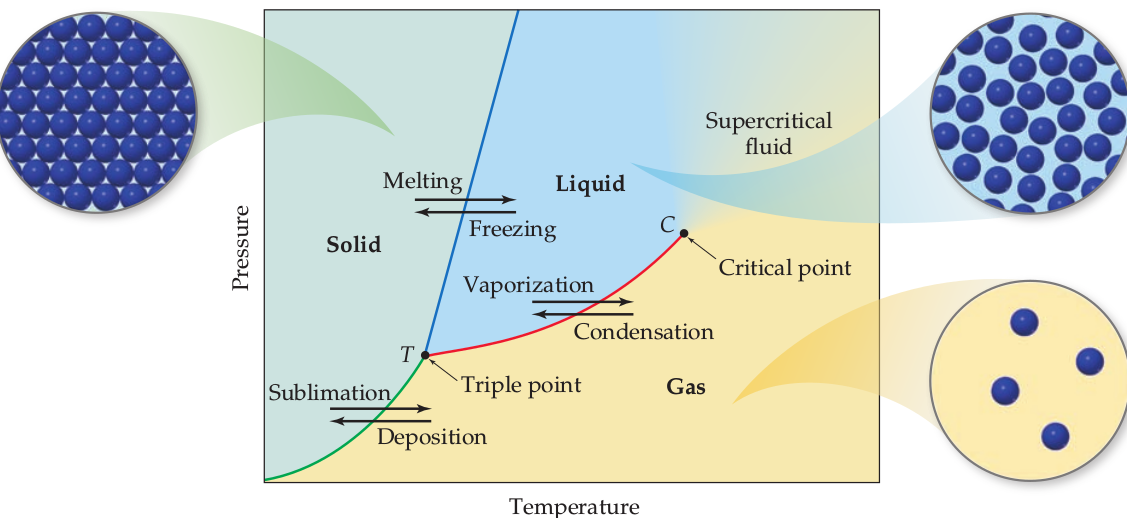
\includegraphics[width=0.75\textwidth]{phase_diagram.png}
\end{figure}

\begin{figure}[H]
\centering
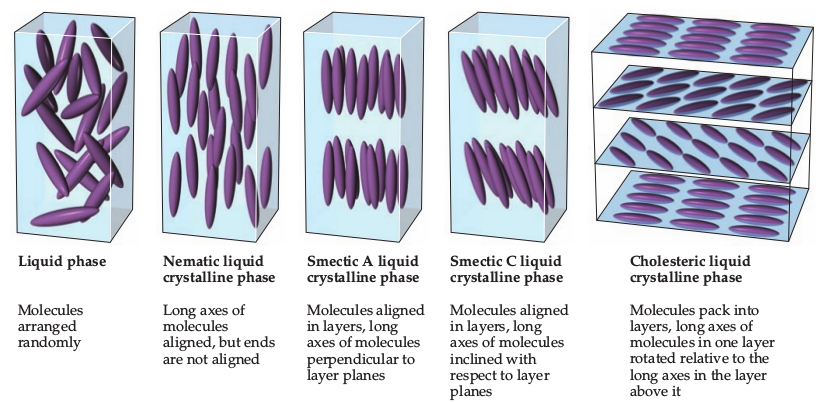
\includegraphics[width=\textwidth]{liquid_crystals.png}
\end{figure}


\end{mdframed}


\begin{mdframed}
\subsection{Intermolecular Forces}
Stronger IMFs mean higher viscosity, surface tension (maintain surface area)
and capillary action.
For molecules of approximately equal mass and size, \textbf{the strength of
intermolecular attractions increases with increasing polarity}.

\begin{tabularx}{\linewidth}{>{\bfseries}l l X X}
    Name & strength & description & \\
    \midrule
    Dispersion & weakest & instantaneous $e^-$ imbalance disrupt neighbors
        & all molecules do it, oblong, heavier = stronger \\
    Dipole-dipole & weak & between dipoles
        & only between polar molecules \\
    Van der Waal's & weak group & includes dispersion, dipole-dipole. Short range
        & repulsive/attractive, stronger = higher BP\\
    Hydrogen bonding & strong & 10\% covalent, mostly electrostatic
        & molecules with \ce{NH}, \ce{OH}, \ce{HF} groups \\
    Ion-dipole & strongest & between polar group and ion
        & example: \ce{H2O} and an ion \\
\end{tabularx}
\end{mdframed}
